\section{Case Studies}\label{sec:case_studies}
In this section, we present two case studies that illustrate the usefulness and the computational advantages of the algorithms.
The first is an anomalous trajectory detection problem in maritime environment. The second is a fault detection problem in an automotive powertrain system.
The automotive application is particularly appealing because the systems involved are getting more and more sophisticated. In a modern vehicle, several highly complex dynamical systems are interconnected and the methods present in literature may fail to cope with this complexity.
In this context, anomaly detection methods derived from control theory lack a proper handling of the hybrid component and most classical machine learning methods lack a dynamical part altogether.

\subsection{Maritime surveillance}
%\subsubsection{Problem description}
This syntectic dataset emulates a maritime surveillance problem, where the goal is to detect suspicious vessels approaching the harbor from sea by looking at their trajectories.
It was developed by Kong and Jones \cite{kong_temporal_2015}, based on the scenarios described in \cite{kowalska_maritime_2012}, for evaluating their inference algorithms, and we use it for for direct comparison purposes.

The trajectories are represented with planar coordinates $x(t)$ and $y(t)$ and were generated using a Dubins' vehicle model with additive Gaussian noise.
Tree types of scenarios, one normal and two anomalous. In the normal scenario, a vessel approaching from sea heads directly towards the port. In the first anomalous scenario, a ship veer to the island and heads to the port next. This scenario is compatible with human trafficking.
In the second anomalous scenario, a boat tries to approach other vessels in the passage between the peninsula and the island and then veers back to the open sea. This scenario is compatible with terrorist activity.
Some sample traces are shown in Figure \ref{fig:naval_sample}.
The dataset is made of 2000 total trajectories, with 1000 normal trajectories and 1000 anomalous.
More details on this dataset can be found in \cite{kong_temporal_2015}.
\begin{figure}
  \centering
  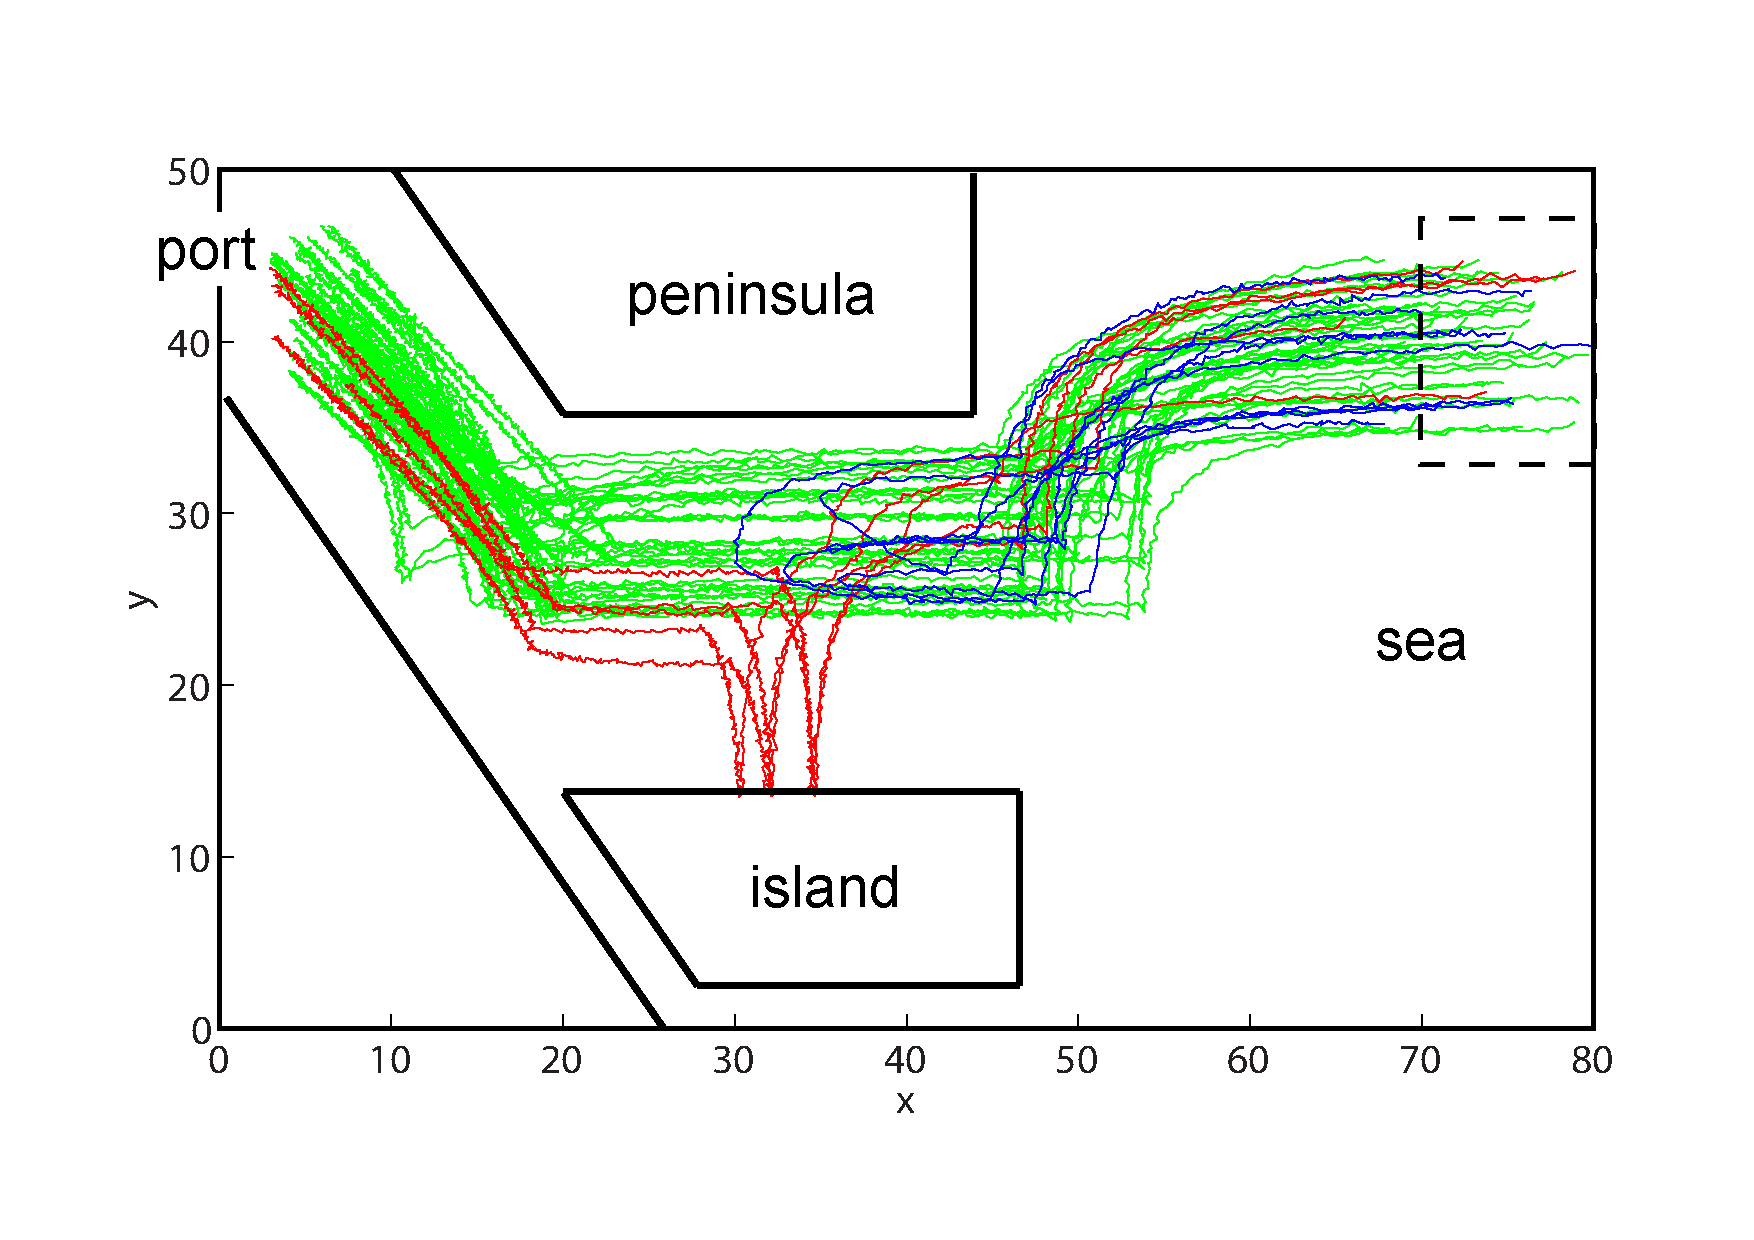
\includegraphics[width=1.0\columnwidth]{naval_sample}
  \caption{Naval surveillance dataset - The vessels behaving normally are shown in green. The red and blue traces represent two types of anomalous paths (human trafficking and terrorism, respectively).}\label{fig:naval_sample}
\end{figure}


\subsection{Fuel control system}
We investigate a fuel control system for a gasoline engine. A model for this system is provided as built-in example in Simulink \cite{SimulinkGuideFTFCS} and we modified it for our purposes.
This model was initially used for Bayesian statistical model checking \cite{zuliani_bayesian_2013} and has been recently proposed as benchmark for the Hybrid Systems community \cite{hoxha_benchmarks_2014}.
We selected this model because it includes all the complexities of real world industrial models, but is still quick to simulate, i.e., it is easy to obtain a large number of trajectories.

\begin{figure}
  \centering
  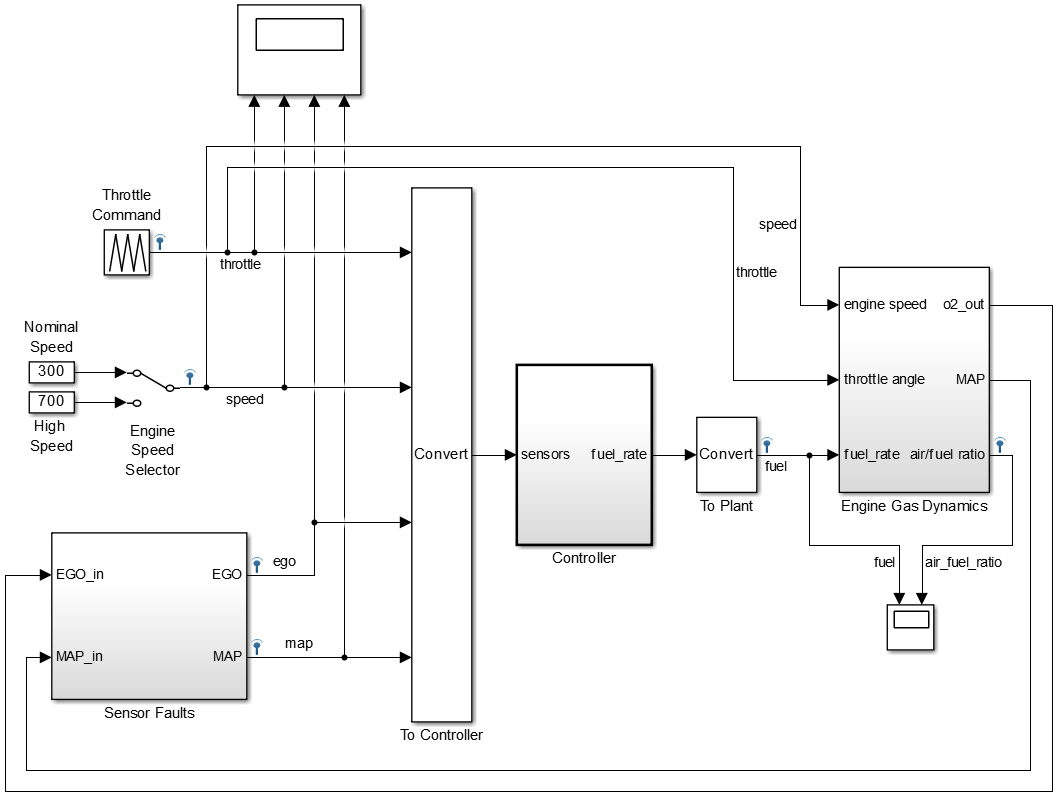
\includegraphics[width=1.0\columnwidth]{fcs_overview}
  \caption{Fuel Control - Overview of the model (modified from \cite{SimulinkGuideFTFCS})}\label{fig:fcs_overview}
\end{figure}
The key quantity in the model is the \emph{air-to-fuel ratio}, that is, the ratio between the mass of air and the mass of fuel in the combustion process. The goal of the control system is to keep it close to the ``ideal'' stoichiometric value for the combustion process.
For this system, the target air-fuel ratio is $14.6$, as it provides a good compromise between power, fuel economy, and emissions. An overview of the Simulink diagram is shown in Figure \ref{fig:fcs_overview}.
There is one main output, the air-to-fuel ratio, one control variable, the fuel rate, and two inputs, the engine speed and the throttle command.
The system estimates the correct fuel rate to achieve the target stoichiometric ratio by taking into account four sensor readings.
Two are related directly to the inputs, the engine speed and the throttle angle. The remaining two sensors provide crucial feedback information: the EGO sensor reports the amount of residual oxygen present in the exhaust gas, and the MAP sensor reports the (intake) manifold absolute pressure.
The EGO value is related to the air-to-fuel ratio, whereas the MAP value is related to the air mass rate.
The diagram in Figure \ref{fig:fcs_overview} is made of several subsystems with different kinds of blocks within, both continuous and discrete, among which there are look-up tables and a Stateflow chart.
Due to these characteristics, this model can exhibit a rich and diverse number of output trajectories, thus making it an interesting candidate for our investigation.

%\subsubsection{Modifications and fault injections}\label{sec:mod_faults}
\begin{figure}
  \centering
  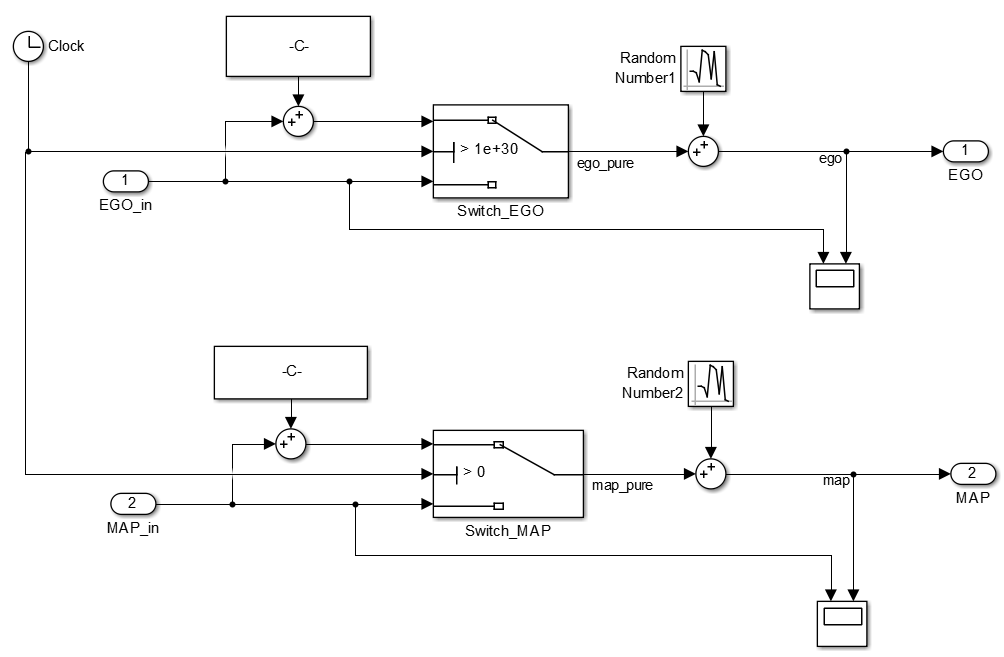
\includegraphics[width=1.0\columnwidth]{fcs_sensorfaults}
  \caption{Fuel Control - Sensor Faults Injection}\label{fig:fcs_sensorfaults}
\end{figure}

The base model, that is, the one included in Simulink, includes a very basic fault detection scheme and fault injection mechanism.
The fault detection scheme is a simple threshold crossing test (within the Stateflow chart), and is only able to detect single off range values. For avoiding the overlap of two anomaly detection schemes, the built-in one has been removed.
In the base model, the faults are injected by simply reporting an incorrect and fixed value for a sensor's reading. Moreover, these faults are always present from the beginning of the simulation. We substituted this simple fault injection mechanism with a more sophisticated unit.
The new subsystem, shown in Figure \ref{fig:fcs_sensorfaults}, is capable of inducing faults in both the EGO and MAP sensors with a \emph{random} arrival time and with a \emph{random} value.
Specifically, the faults can manifest at anytime during the execution (uniformly at random) and the readings of the sensors affected 
%by a fault 
are offset by a value that \emph{varies} at every execution.
Finally, independent Gaussian noise signals, with zero mean and variance $\sigma^2 = 0.01$, have been added at the output of the sensors. 
% and for the initial conditions of the system.

%\subsubsection{Dataset generation}\label{sec:datasets}
For the fuel control system, $1200$ total simulations were performed.
In all cases, the throttle command provides a periodic triangular input, and the engine speed is kept constant at $300$ rad/sec ($2865$ RPM). The simulation time is $60$ seconds. In details, we obtained:
\begin{itemize}
\item 600 traces where the system was working normally;
\item 200 traces with a fault in the EGO sensor;
\item 200 traces with a fault in the MAP sensor;
\item 200 traces with faults in both sensors.
\end{itemize}
For every trace we collected the values of the air-to-fuel ratio ($x_1$), the fuel rate ($x_2$), and the EGO and MAP sensors' readings  ($x_3$ and $x_4$).
The average simulation time for obtaining a single trace was roughly $1$ second. 